\documentclass[12pt,a4paper]{report}
\usepackage[utf8x]{inputenc}
\usepackage[portuguese]{babel}
\usepackage{graphicx}
\usepackage{float}
\usepackage{minted}

\begin{document}
\setminted{fontsize=\footnotesize,baselinestretch=1}

\title{Relatório Trabalho Prático LI1 \paragraph{}\textbf{"Micro Machines"}}

\begin{figure}[t]

\includegraphics[scale=0.7]{ee-um.png}
\end{figure}

\author{Grupo 77\\
\\
Francisco Peixoto e Maria Miguel Regueiras}
\date{Braga, 20 de Dezembro 2017}
\maketitle
\tableofcontents
\listoffigures

\chapter{Introdução}

  \section{Contextualização}
  \paragraph{} Este trabalho prático, realizado no âmbito da unidade curricular de Laboratórios de Informática 1, teve como objetivo o desenvolvimento do jogo \textit{Micro Machines} na linguagem de programação \textit{Haskell}. 

  

  \section{Motivação}
  \paragraph{} O trabalho em si teve grande importância para os membros do grupo a vários níveis, já que permitiu o desenvolvimento do trabalho em equipa e, individualmente, contribuiu para a melhor compreensão da linguagem em questão.
  
  
  \section{Objectivos}
  \paragraph{} Sumariamente, este projeto teve como objetivos a aprendizagem da linguagem em causa, assim como o desenvolvimento do pensamento lógico e crítico aplicado à programação e aos os seus paradigmas. Também visou a cooperação entre os membros do grupo e o a ultilização do \textit{SVN}.

%---------------------------------------------------------------%

\chapter{Análise de Requisitos}
\paragraph{} O trabalho encontra-se dividido em duas partes fulcrais : a \textit{Fase 1} e a \textit{Fase 2}. Estas, por sua vez, estão também divididas, cada uma em três \textit{Tarefas}. 
\newline Uma \textit{Tarefa} apresenta diferentes problemas com o objetivo de simplificar o desenvolvimento do jogo.

%--
\section{Fase 1}
\label{sec:analisefase1}
\paragraph{} Na primeira fase encontramos, tal como referido em cima, três Tarefas:

\begin{enumerate}
 \item[]
\includegraphics[scale=0.7]{p1.png}  \textbf{Tarefa 1} - Construir Mapas  

   \begin{itemize}
   \item Construir \textit{Mapas} a partir de \textit{Caminhos}, isto é, a partir de um conjunto de \textit{Passos} como "Avança", "Curva Dir", "Sobe", entre outros.
   \end{itemize}

 \item[]
\includegraphics[scale=0.7]{p1.png}  \textbf{Tarefa 2} - Validar Mapas

   \begin{itemize}
   \item O nome da Tarefa é bastante objetivo, resume-se a verificar se um \textit{Mapa} é válido ou não tendo em consideração um conjunto de restrições/regras.
   \end{itemize}
   
 \item[]
\includegraphics[scale=0.7]{p1.png}  \textbf{Tarefa 3} - Movimentar o Carro

    \begin{itemize}
    \item Focando agora no carro em si, esta Tarefa visa movimentar o \textit{Carro} e definir as possíveis interações com o \textit{Mapa}, como por exemplo, colisões.
    \end{itemize}
    
\end{enumerate}

%--
\newpage
\section{Fase 2}
\label{sec:analisefase2}
\paragraph{}Dando continuação à Fase 1, na Fase 2 estão presentes mais três Tarefas:

\begin{enumerate}

 \item[]
\includegraphics[scale=0.7]{p1.png} \textbf{Tarefa 4} - Atualizar o Estado
 
    \begin{itemize}
    \item Introduzindo dois novos tipos de dados, \textit{Jogo} e \textit{Ação}, o objetivo desta Tarefa é atualizar o \textit{Estado} interno do \textit{Jogo} dado uma \textit{Ação} realizada pelo jogador.
    \end{itemize}
 
 \item[]
\includegraphics[scale=0.7]{p1.png} \textbf{Tarefa 5} - Implementação do Jogo em \textit{Gloss}
 
     \begin{itemize}
     \item Usando a biblioteca \textit{Gloss} que permite ao programador desenvolver animações, simulações e desenho gráfico, implementar a componente gráfica do jogo complementando-a com a junção de todas as Tarefas previamente resolvidas.
     \end{itemize}
 
 \item[]
\includegraphics[scale=0.7]{p1.png} \textbf{Tarefa 6} - 
Implementar uma Estratégia de Corrida 

     \begin{itemize}
     \item Por fim, é proposto a criação de um \textit{bot} com o intuito de implementar uma estratégia de corrida para competir com \textit{bots} desenvolvidos pelos docentes da UC e pelos colegas num torneio.
     \end{itemize}
      
      
\end{enumerate}

%---------------------------------------------------------------%

\chapter{A Nossa Solução}
\label{sec:solucao}
 
 \paragraph{}Com os objetivos de cada Fase em consideração, o grupo chegou a soluções plausíveis e executáveis para cada Tarefa. O processo foi longo e com obstáculos mas, em suma, aqui se apresentam as respetivas resoluções desenvolvidas para cada Tarefa (dadas as informações da biblioteca "LI11718.hs", fornecida pelos docentes da UC).
 
 %--
 \section{Tarefa 1 - Construir Mapas}
 \label{Tarefa1_2017li1g77}
 
 \paragraph{}\textbf{Função Objetivo:}
 \begin{minted}{haskell}
 constroi ::  Caminho -> Mapa
 \end{minted}
 
\paragraph{}Tendo em conta que um \textit{Caminho} é um conjunto de \textit{Passos}
e um \textit{Mapa} assume a seguinte forma : 
\begin{minted}{haskell}
(Mapa (Posicao Inicial, Orientacao Inicial) Tabuleiro)
\end{minted}

Ora, com isto, foram necessárias duas funções essenciais para:
\begin{itemize}
\item[]
\includegraphics[scale=0.7]{p4.png} Obter a Posição Inicial;
\item[]
\includegraphics[scale=0.7]{p4.png} Obter o Tabuleiro.
\end{itemize}

\paragraph{}A primeira função (posição inicial) já nos era fornecida na biblioteca (a função \textbf{partida}). Para além disso, como referido no enunciado, a orientação inicial seria sempre \textbf{Este}.
\paragraph{} 
\paragraph{}Assim, tentou-se converter um \textit{Passo} numa \textit{Peça} através da função \textbf{iPeca} de forma a começar a construir o \textit{Tabuleiro}.
\paragraph{}Seguidamente, essa \textit{Peça} teria de ser inserida num \textit{Tabuleiro} vazio, isto é, um \textit{Tabuleiro} apenas constituído por peças do tipo "Lava". 
\newline Para isso foi necessário criar uma função que originasse um \textit{Tabuleiro} deste carácter, a função \textbf{tabVazio}. 
\newline Concluindo a primeira parte, a função \textbf{iTabuleiro} tem como propósito inserir uma só \textit{Peça} no \textit{Tabuleiro} vazio (com ajuda de funções auxiliares):


\begin{minted}{haskell}
iTabuleiro:: Passo-> Altura-> Orientacao-> Posicao-> Tabuleiro-> Tabuleiro 
iTabuleiro p a o (x,y) (h:r) 
    | y==0 = subx x h (iPeca p a o) :r
    | otherwise =  h : iTabuleiro p a o (x,y-1) r
\end{minted}


\paragraph{}Contudo, um \textit{Caminho} é constituído por vários passos e, por conseguinte, várias \textit{Peças} se originam. Então, foram desenvolvidas funções que calculassem a posição, a orientação e a altura seguintes da \textit{Peça} ou do \textit{Passo} em questão para conseguir converter o \textit{Caminho} completo. Estas são a \textbf{iPosicao} e a \textbf{auxPeca}. 

\paragraph{}Por fim, criou-se a função \textbf{iTabuleiros} que é a junção de todas as funções direcionadas para a criação do \textit{Tabuleiro} com todas as \textit{Peças} inseridas conforme o \textit{Caminho} dado:

\begin{minted}{haskell}

iTabuleiros:: Caminho-> Altura-> Orientacao-> Posicao-> Tabuleiro-> Tabuleiro 
iTabuleiros [] a o p t = t
iTabuleiros (x:xs) a o p t = iTabuleiros xs a' o' p' (iTabuleiro x a o p t)   
                   where 
                    a' = fst(auxPeca x a o)  
                    o' = snd(auxPeca x a o) 
                    p' = iPosicao x o p
\end{minted}

\paragraph{}\textbf{Função Objetivo sugerida:}

\begin{minted}{haskell}
constroi :: Caminho -> Mapa 
constroi [] = Mapa (partida [], Este) (tabVazio(dimensao []))
constroi c =
Mapa (partida c, Este) (iTabuleiros c 0 Este (partida c) (tabVazio(dimensao c)))
\end{minted}

%--
\newpage
\section{Tarefa 2 - Validar Mapas}
\label{Tarefa2_2017li1g77}

\paragraph{}\textbf{Função Objetivo:}

\begin{minted}{haskell}
valida :: Mapa -> Bool
\end{minted}
 

\paragraph{}Para validar um \textit{Mapa} há um conjunto de regras que devemos ter em consideração, segundo o enunciado fornecido pelos docentes da UC. Assim, o grupo tomou a iniciativa de dividir este problema em três partes essenciais:

\begin{enumerate}
\item A validação de aspetos relacionados apenas com o \textit{Tabuleiro};
\item A validação de aspetos relacionados apenas com a \textit{Peça} de Partida;
\item A validação de aspetos relacionados apenas com o \textit{Percurso}.
\end{enumerate}

\paragraph{}\textbf{Validação do Tabuleiro}
\paragraph{}Existem quatro regras principais para um \textit{Tabuleiro} ser válido:

\begin{itemize}
\item[]
\includegraphics[scale=0.7]{p4.png} Apresentar um formato regular;
\item[]
\includegraphics[scale=0.7]{p4.png} A moldura deve ser constituída apenas por \textit{Peças} do tipo "Lava";
\item[]
\includegraphics[scale=0.7]{p4.png} Não pode ser constituído apenas por \textit{Peças} do tipo "Lava";
\item[]
\includegraphics[scale=0.7]{p4.png} Todas as \textit{Peças} do tipo "Lava" têm de possuir altura igual a zero.
\end{itemize}

\paragraph{} Para verificar o primeiro aspeto, o grupo desenvolveu a função \textbf{vFormatoTabuleiro} que, resumidamente, verifica se existem o mesmo número de colunas e linhas.
\newline Em relação ao segundo, terceiro e quarto pontos, foram criadas as funçôes \textbf{vMoldura}, \textbf{nValidaTabLava}, \textbf{vAltLava}.

\paragraph{} A função final que junta todas as funções referidas, \textbf{vBases}, é dada por:
 \begin{minted}{haskell}
vBases :: Mapa -> Bool                                            
vBases ( Mapa (p,o) tab) = vFT && vM && nVTL && vAL
   where
     vFT  = vFormatoTabuleiro tab
     vM   = vMoldura tab
     nVTL = nValidaTabLava tab
     vAL  = vAltLava tab
 \end{minted}

\paragraph{}\textbf{Validação da Peça de Partida}

\paragraph{} Para validar a \textit{Peça} de Partida é preciso ter em mente que:

 \begin{itemize}
 \item[]
\includegraphics[scale=0.7]{p4.png} A orientação inicial tem de ser compatível com \textit{Peça};
 \item[]
\includegraphics[scale=0.7]{p4.png} Não pode ser uma \textit{Peça} do tipo "Lava".
 \end{itemize}
 
 \paragraph{}Assim, desenvolveram-se duas funções, primeiro uma função simples que só verifica se a \textit{Peça} não é do tipo "Lava", a função \textbf{vPosicaoInicial}.
 \newline De seguida, a função \textbf{vOrientacaoPPartida} que verifica todas as opções possíveis e determina se a orientação é compatível com a \textit{Peça} de Partida.
 \paragraph{}A função final que junta todas as funções referidas, \textbf{vInicio}, é dada por:
 
 \begin{minted}{haskell}
vInicio :: Mapa -> Bool
vInicio m  = vOrientacaoPPartida m && vPosicaoInicial m
 \end{minted}
 
\paragraph{}\textbf{Validação do Percurso}
\paragraph{}Ao abordar este ponto, o grupo decidiu criar um novo tipo, o tipo \textit{Percurso} de forma a facilitar a compreensão de quem lê o código e o desenvolvimento da \textit{Tarefa} por parte do grupo. 
\newline Este novo tipo consiste num par de listas de \textit{Posições} e \textit{Peças} correspondentes a uma trajetória.

\begin{minted}{haskell}
type Percurso = ([Posicao],[Peca])
\end{minted}

\paragraph{}Para validar o \textit{Percurso} existem três restrições principais:

  \begin{itemize}
  \item[]
\includegraphics[scale=0.7]{p4.png} A trajetória tem de ser válida;
  \item[]
\includegraphics[scale=0.7]{p4.png} As alturas do percurso têm de ser compatíveis entre si, assim como as \textit{Peças};
  \item[]
\includegraphics[scale=0.7]{p4.png} Todas as \textit{Peças} fora do \textit{Percurso} têm de ser do tipo "Lava".
  \end{itemize}

\paragraph{} De forma resumida, antes de tudo, foi essencial desenvolver uma forma de arranjar o \textit{Percurso} a partir do \textit{Mapa} em si, a função \textbf{iPercurso} resolveu a questão (recorrendo a funções auxiliares): 
 
 \begin{minted}{haskell}
iPercurso :: Mapa -> Percurso                           
iPercurso (Mapa (p,o) t) = if notlava p t
                     then auxPercurso p o t ([],[]) 
                           else ([p],[Peca Lava 0])
 \end{minted}
 
\paragraph{} De maneira a resolver o primeiro ponto, foi criada a função \textbf{vTrajetoria} que verifica se uma Tragetória de um Percurso é válida, ou seja, se o primeiro e a último par Posição/Peça são iguais e diferentes de Lava.
\newline Seguidamente, em relação ao segundo ponto, criou-se a função \textbf{vAltura} que não só verifica as alturas das \textit{Peças} como também verifica se estas são compatíveis entre si.
\newline Por fim, a função \textbf{vResto} certifica-se que tudo que não pertença ao \textit{Percurso} é do tipo "Lava".

A função que junta todas as funções referidas, \textbf{vPercurso}, é dada por:
 \begin{minted}{haskell}
vPercurso :: Mapa -> Bool
vPercurso m = vTrajetoria m && vResto m && vAltura m
 \end{minted}

\paragraph{}\textbf{Função Objetivo sugerida:}

\begin{minted}{haskell}
valida :: Mapa -> Bool
valida m = vBases  m && vInicio m && vPercurso m 
\end{minted}


%--
\newpage
\section{Tarefa 3 - Movimentar o Carro}
\label{Tarefa3_2017li1g77}

\paragraph{}\textbf{Função Objetivo:}

\begin{minted}{haskell}
movimenta :: Tabuleiro -> Tempo -> Carro -> Maybe Carro
\end{minted}

\paragraph{} Para mover o \textit{Carro}, o grupo encontrou alguns contratempos durante a Fase 1. Contudo, chegou a uma solução executável embora simplista.

\paragraph{} Dadas as informações do \textit{Carro}, foi necessário compreender como este se comportava e foi claro que este iria sofrer \textit{colisões} com as paredes de alturas diferentes, com \textit{Peças} do tipo "Curva" e que quando se encontrava numa do tipo "Lava" era prejudicado.

\paragraph{}Primeiramente, foi essencial definir uma função que movesse efetivamente o \textit{Carro}, a função \textbf{move}.
\newline Assim, foi importante saber onde este estaria a entrar numa \textit{Peça} do tipo "Curva", dado que existem duas formas possíveis de entrar e, por conseguinte, se estaria a virar à direita ou à esquerda. Criaram-se, então, as funções \textbf{vEsquerda} e \textbf{vDireita} que verificam para que lado está o \textit{Carro} a virar.
\paragraph{} Sabendo agora para que lado está a virar, definiu-se uma função que dita o que acontece em cada \textit{Peça} do Tabuleiro e devolve o novo \textit{Estado} do \textit{Carro}, a função \textbf{iPartida} (que devolve \textit{Nothing} quando este cai à "Lava" e \textit{Just Carro} com as devidas alterações para as outras \textit{Peças}).

\paragraph{} Por fim, foi necessário definir o que acontece durante todo o tempo dado, assim definiu-se a função \textbf{i} que funciona como função auxiliar para a função final.

\paragraph{}\textbf{Função Objetivo sugerida:}

\begin{minted}{haskell}
movimenta :: Tabuleiro -> Tempo -> Carro -> Maybe Carro
movimenta tab t (Carro (x,y) d vl) = i tab (Just (Carro (x,y) d vl)) t 
\end{minted}


%--
\newpage
\section{Tarefa 4 - Atualizar Estado}
\label{Tarefa4_2017li1g77}

\paragraph{}\textbf{Função Objetivo:}

\begin{minted}{haskell}
atualiza :: Tempo -> Jogo -> Int -> Acao -> Jogo
\end{minted}

De modo a atualizar o \textit{Estado} do \textit{Jogo} dadas as \textit{Ações} do jogador estão implicitas várias componentes.
\newline Num \textit{Jogo} há 3 partes que necessitam atualização:

\begin{itemize}
\item[]
\includegraphics[scale=0.7]{p2.png} O \textit{Histórico}.
\item[]
\includegraphics[scale=0.7]{p2.png} A lista de tempos dos \textit{Nitros};
\item[]
\includegraphics[scale=0.7]{p2.png} A lista de \textit{Carros};
\end{itemize}
 
\paragraph{}\textbf{Atualizar o Histórico}

\paragraph{} De forma a atualizar o \textit{Histórico}, foi necessário verificar se a \textit{Posição} onde o \textit{Carro} se encontra já existe na lista, se a posição já fizer parte da lista, esta mantêm-se igual, caso não se encontre adiciona-se a respetiva posição à cabeça da lista. Isto através da função \textbf{ihistorico}.

\paragraph{}\textbf{Atualizar os Nitros}

\paragraph{} Já para atualizar a lista de tempos dos \textit{Nitros}, apenas foi preciso identificar o jogador que está a utilizar o \textit{Nitro} e retirar o tempo que foi usado ao jogador respetivo, através da função \textbf{iNitro}.

\paragraph{}\textbf{Atualizar o Carro}

\paragraph{} Por fim, de modo a atualizar os \textit{Carros} existem alguns pontos a ter em consideração, como a \textit{Direção} e a \textit{Velocidade}. No \textit{Jogo} são fornecidas as \textit{Propriedades} da pista, ou seja, valores que se devem aplicar ao \textit{Carro}. Todas são constantes exceto o atrito que é uma percentagem. Assim, através de fórmulas, cálculos de vetores, entre outros processos se desenvolveram as seguintes funções:

\begin{enumerate}
\item Direção 
\newline Componente que se atualiza tendo em conta para que lado o \textit{Carro} está a virar e a constante k\textunderscore roda através da função \textbf{virar} que aplica a constante e confirma se este está a virar ou não.
\item Velocidade
\newline Para esta componente, primeiramente, aplicaram-se as constantes k\textunderscore atrito e k\textunderscore pneus à velociade inicial pela função \textbf{fIniciais}. Depois foram desenvolvidas funções que aplicassem o resto das constantes dependendo das \textit{Ações} realizadas pelo jogador: \textbf{fGrav} que aplica a constante k\textunderscore peso apenas nas \textit{Peças} do tipo "Rampa"; \textbf{fAcel} que aplica a constante k\textunderscore acel sempre que o \textit{Carro} acelera; \textbf{fNitro} que aplica nitro no jogador indicado na \textit{Ação}.
\newline A função que realiza primeiro a \textbf{fIniciais} e só depois todas as outras mencionadas é a função \textbf{forcas}.
\end{enumerate}

\paragraph{}\textbf{Função Objetivo sugerida:}

\begin{minted}{haskell}
atualiza :: Tempo -> Jogo -> Int -> Acao -> Jogo
atualiza t (Jogo m p c lN lH) jogador acao = Jogo m p carros nitros historico
                   where
                       carros    = (forcas jogador (Jogo m p c lN lH) t acao)
                       nitros    = (initro t (Jogo m p c lN lH) acao jogador )
                       historico = (ihistorico (Jogo m p c lN lH) jogador)

\end{minted}


%--
\newpage
\section{Tarefa 5 - Implementação do Jogo em \textit{Gloss}}
\label{Tarefa5_2017li1g77}

\paragraph{} Na \textit{Tarefa} que se segue o grupo teve a liberdade de explorar a biblioteca \textit{Gloss} e desenvolver a componente gráfica do jogo. 
\newline O modelo final tem alguns erros que o grupo não conseguiu resolver, contudo implementaram-se  algumas funcionalidades interessantes que tornam o jogo mais apelativo.

\paragraph{} O tema escolhido foi baseado nos filmes da saga "Star Wars" e, em vez de um jogo de carros, criou-se um jogo de corridas de \textit{naves} espaciais: 

\begin{figure}[H]
\caption{Naves}
\centering

\includegraphics[scale = 4]{naveAzul.png}
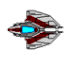
\includegraphics[scale = 4]{naveVermelha.png}
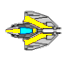
\includegraphics[scale = 4]{naveAmarela.png}
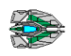
\includegraphics[scale = 4]{naveVerde.png}
\end{figure}


\paragraph{} Ao abrir o executável da \textit{Tarefa}, a janela abre em \textit{Full Screen} um menu que permite ao jogador escolher de entre três \textit{Mapas} um onde quer jogar (através das teclas F1, F2 e F3): um de lava, um de areia e um de gelo.

\begin{figure}[H]
\caption{Menu Inicial}
\centering
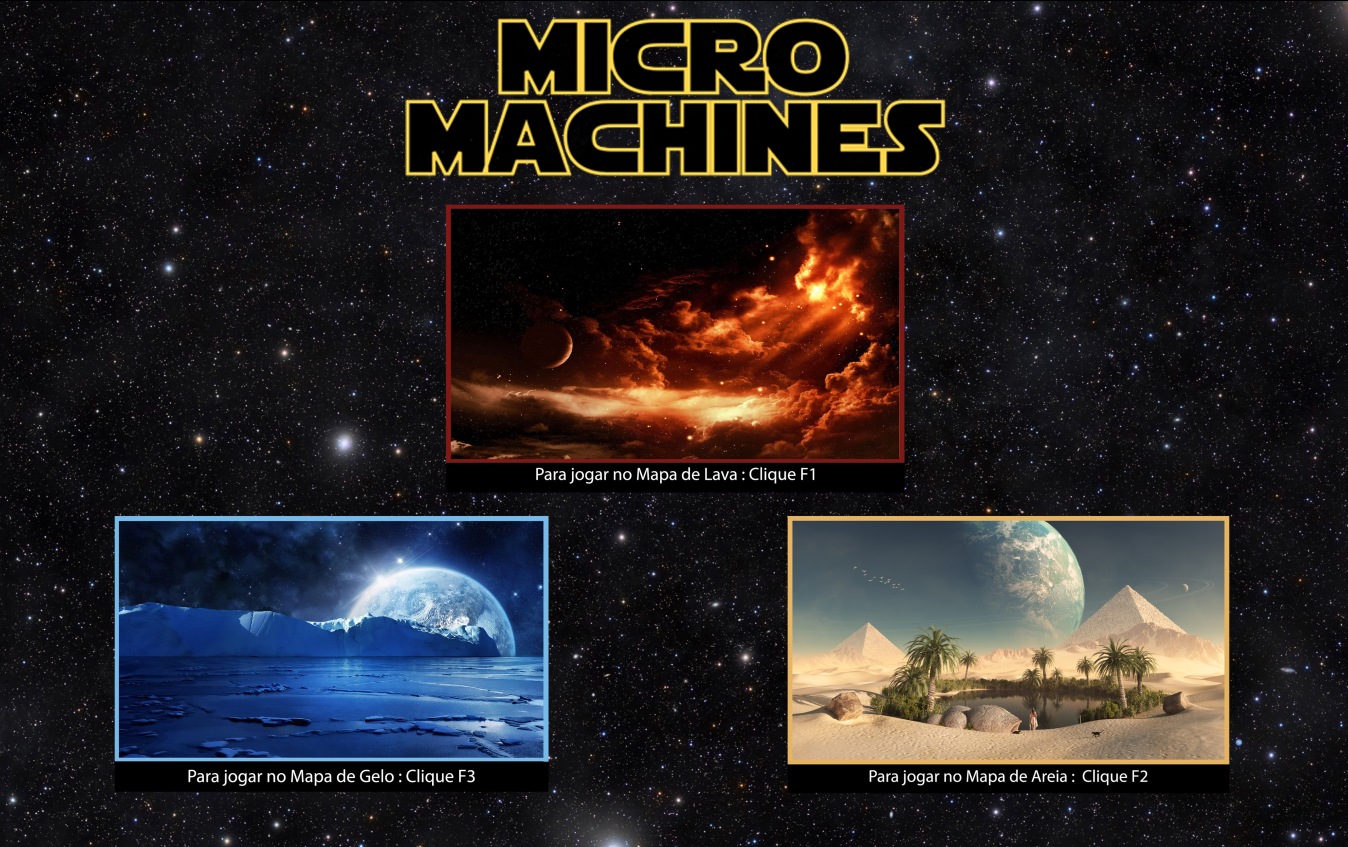
\includegraphics[scale = 0.27]{menu.png}
\end{figure}

\paragraph{} É de notar que é possível mudar de \textit{Mapa} sem voltar ao menu inicial e que os \textit{Mapas} têm  \textit{Propriedades} diferentes. 
\paragraph{} Para cada \textit{Mapa} foram criadas diferentes imagens para as \textit{Peças}, por exemplo, no \textit{Mapa} de gelo encontramos as imagens seguintes:

\begin{figure}[H]
\caption{Peças do mundo de gelo}
\centering

\includegraphics[scale = 0.5]{agua.png}

\includegraphics[scale = 0.5]{aguacurva.png}

\includegraphics[scale = 0.51]{gelo.png}
\end{figure}
De forma a transformar a informação contida no \textit{Tabuleiro} numa imagem no ecrã, criou-se a função \textbf{tabpic} que resulta de uma combinação de funções auxiliares, que têm como intuito moldar os vários tipos existentes, como por exemplo as "linhas" de \textit{Peças}.

\begin{figure}[H]
\centering
\caption{Exemplo de um Tabuleiro}
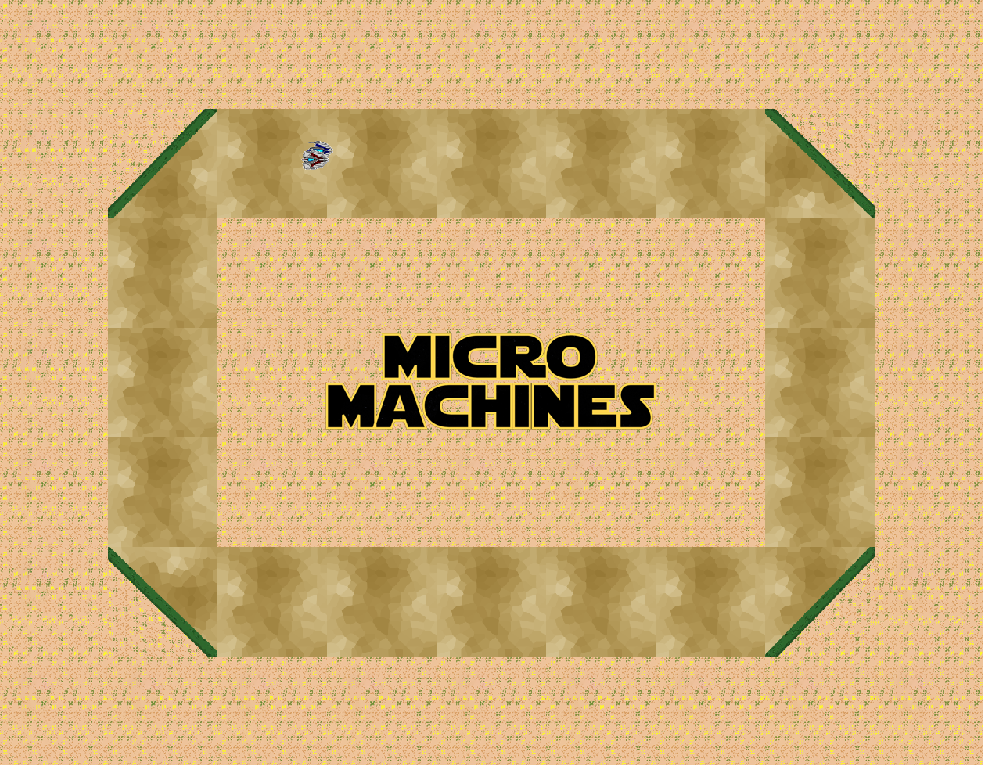
\includegraphics[scale = 0.35]{modoareia.png}
\end{figure}

\paragraph{} Para desenvolver a mecânica do jogo, começou por se definir o tipo \textit{Estado}:

\begin{minted}{haskell}
type Estado = (Int, Jogo, Acao, Picture, Picture, [Picture], [Picture], [Picture])
\end{minted}

\paragraph{} O \textit{Estado} constitui a base da \textit{Tarefa}, já que permite o funcionamento da função do Gloss \textbf{play}, que trabalha segundo os seguintes componentes: 

\begin{minted}{haskell}
play = Display -> Color -> Int 
       -> estadoInicial -> desenhaEstado -> reageEvento -> reageTempo -> IO ()
\end{minted}

\paragraph{} Primeiramente, foi necessário criar um estado inicial. Por isso, a função \textbf{estadoInicial} contêm as informações necessárias para começar um jogo imprimindo no ecrã uma imagem composta.
\paragraph{} De seguida, foi essencial converter o \textit{Estado} atualizado em outputs gráficos, para isso criou-se a função \textbf{desenhaEstado}, que permite obter o jogo pretendido consoante o \textit{Mapa} desejado.
\paragraph{} Já para receber inputs do Utilizador, o grupo desenvolveu a função \textbf{reageEvento} que gera \textit{Estados} do jogo atualizados respetivamente.
\paragraph{} Por fim, de modo a atualizar o \textit{Estado} em si, desenvolveu-se a função \textbf{reageTempo} que altera o \textit{Jogo} segundo a função \textbf{atualizaMovimenta} (junção da função " \textit{atualiza} " e da função " \textbf{movimenta} " correspondentes à \textit{Tarefa} 4, ver \ref{Tarefa4_2017li1g77}, e à \textit{Tarefa} 3, ver \ref{Tarefa3_2017li1g77}, respetivamente)
\paragraph{} É de notar que o \textbf{Jogo} permite apenas um \textit{Jogador} que compete contra 3 \textit{bots}, criados pelo grupo para a \textit{Tarefa} 6.

%--
\newpage
\section{Tarefa 6 - Implementar uma Estratégia de Corrida }
\label{Tarefa6_2017li1g77}

\paragraph{}\textbf{Função Objetivo:}

\begin{minted}{haskell}
bot :: Tempo -> Jogo -> Int -> Acao
\end{minted}

\paragraph{} A \textit{Tarefa} 6 consistiu na criação de um bot, que percorre um dado \textit{Mapa} segundo as \textit{Ações} ponderadas pelo Grupo.

\paragraph{} Primeiramente, com recurso ao tipo \textit{Percurso} (ver \ref{Tarefa2_2017li1g77}) o \textit{bot} identifica por onde se vai movimentar, tendo em atenção a \textit{Peça} atual e a \textit{Peça} futura. De modo a analisar as \textit{peças} relevantes, o grupo elaborou as funções \textbf{pecaAtual} e a \textbf{pecaFutura}, que identificam as \textit{Peças} respetivamente.

\paragraph{} Mais tarde, foi necessária as funções \textbf{muda} e \textbf{identifica} para identificar no \textit{Percurso} a \textit{Posição/Peça} onde se encontra o \textit{Carro}.

\paragraph{} Por fim, as funções \textbf{curvaNO}, \textbf{retaNITRO} e \textbf{curvaYES} atribuem \textit{Ações} consoante a \textit{velocidade} do \textit{Carro}, de forma a garantir uma boa performance no percurso, com base nas \textit{Peças}.

\paragraph{}\textbf{Função Objetivo sugerida:}

\begin{minted}{haskell}
bot :: Tempo -> Jogo -> Int -> Acao
bot tick (Jogo mapa p c n h) i 
 | vel0 c i = curvaYES i (pecaAtual percurso) (pecaFutura percurso) c
 | vel1 c i = retaNITRO i (pecaAtual percurso) (pecaFutura percurso) c
 | otherwise = curvaNO i (pecaAtual percurso) (pecaFutura percurso) c
                                 where percurso = muda i (iPercurso mapa) c
\end{minted}

%--------------------------------------------------------------%
\newpage
\chapter{Validação da Solução}

\paragraph{} Para validar a solução do grupo, em cada Tarefa foram realizadas diferentes formas de testar:

\begin{itemize}

\item[]
\includegraphics[scale=0.7]{p3.png} Para a \textbf{Tarefa 1} e para a \textbf{Tarefa 2} (ver \ref{Tarefa1_2017li1g77}  e \ref{Tarefa2_2017li1g77}) foram realizados testes que iriam ser verificados no oráculo criado pelos docentes.

\item[]
\includegraphics[scale=0.7]{p3.png} Na \textbf{Tarefa 3} (ver \ref{Tarefa3_2017li1g77}), para além dos testes que se criaram para a posterior verificação do oráculo, desenvolveu-se uma função auxiliar, a função \textbf{m}, que facilitou a realização e a leitura dos testes por parte do grupo.
\item[]
\includegraphics[scale=0.7]{p3.png} \textbf{Tarefa 4} (ver \ref{Tarefa4_2017li1g77}) o grupo também escolheu criar funções que facilitassem a sua validação, as funções \textbf{a0}, \textbf{a1}, \textbf{a2} e \textbf{a3}, cada uma referindo-se ao jogador em causa. 

\item[]
\includegraphics[scale=0.7]{p3.png} Para validar a \textbf{Tarefa 5} (ver \ref{Tarefa5_2017li1g77}) o grupo testou o executável criado e foi ajustando os eventuais problemas.

\item[]
\includegraphics[scale=0.7]{p3.png} Finalmente, na \textbf{Tarefa 6} (ver \ref{Tarefa6_2017li1g77}) usou-se o torneio e tendo em conta as corridas que se iam realizando fez-se ajustes às funções conforme o comportamento do \textit{Carro}.


\end{itemize}

%--------------------------------------------------------------%
\newpage
\chapter{Conclusão}
\paragraph{} Em suma, elaborar este projeto contribuiu não só para a aprendizagem da Linguagem \textit{Haskell}, mas também alargou os nossos conhecimentos no que toca à cooperação em grupo e ao uso do \textit{SVN}.
\paragraph{} Para além disso, sentimos que este trabalho contribuiu de forma positiva para nos mostrar outras vertentes de uma linguagem funcional (neste caso \textit{Haskell}), como é o caso do \textit{Gloss}, que nos ajudou na elaboração da interface gráfica. 


\bibliographystyle{plain}
\bibliography{document}  


\end{document}